\documentclass[../lecture-notes-148x210.tex]{subfiles}

\begin{document}

\begin{definition}
    A cryptographic commitment scheme allows one party to commit to a chosen statement (such as a value, vector, or polynomial) without revealing the statement itself. The commitment can be revealed in full or in part at a later time, ensuring the integrity and secrecy of the original statement until the moment of disclosure.
\end{definition}

Before delving into the details, here is the intuition of cryptographic commitments.

Imagine putting a letter with some message into a box and locking it with your key. 
You then give that box to your friend, who cannot open it without the key.
In this scenario, you have made a commitment to the message inside the box. 
You cannot change the content of the letter, as it is in your friend's possession. 
At the same time, your friend cannot access the letter since they do not have the key to unlock the box.

\begin{figure}[H]
    \centering
    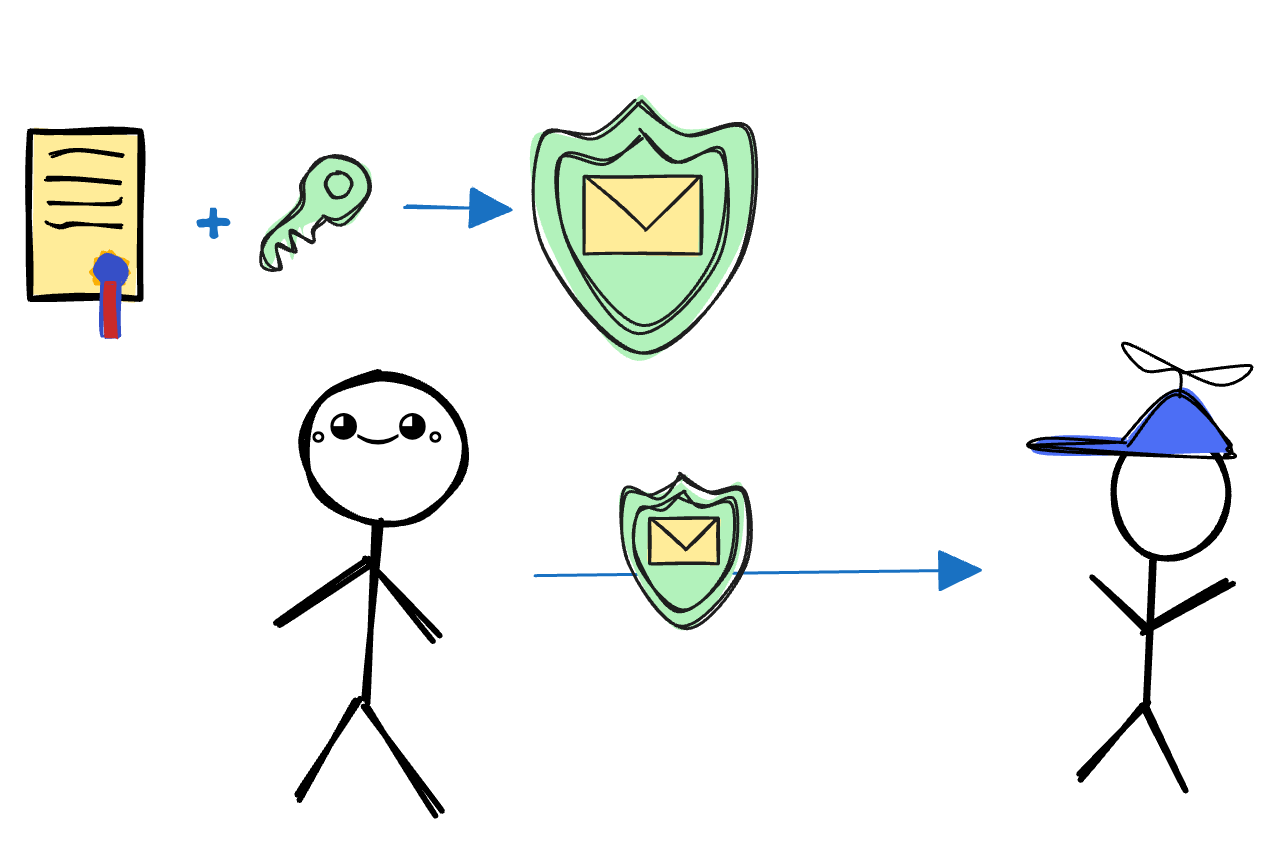
\includegraphics[width=0.5\linewidth, clip]{images/lecture_5/CommitmentExample.png}

    \caption{Commitment scheme}
\end{figure}

\begin{definition}[Commitment Scheme]
    
    Commitment Scheme $\Pi_{\text{commitment}}$ is a tuple of three algorithms: $\Pi_{\text{commitment}} = (\mathsf{Setup}, \mathsf{Commit}, \mathsf{Verify})$.

    \begin{enumerate}

        \item $\mathsf{Setup} (1^{\lambda})$: returns public parameter $\mathsf{pp}$ for both comitter and verifier;

        \item  $\mathsf{Commit} (\mathsf{pp}, m)$: returns a commitment $c$ to the message $m$ using public parameters $\mathsf{pp}$ and, optionally, a secret opening hint $r$;

        \item  $\mathsf{Open} (\mathsf{pp}, c, m, r)$: verifies the opening of the commitment $c$ to the message $m$ with an opening hint $r$. 
    \end{enumerate}
\end{definition}

\begin{definition}[Commitment Scheme]
    Properties of commitment schemes:
    \begin{enumerate}
        \item \textit{Hiding: } verifier should not learn any information about the message given only the commitment $c$. To put it formally, we define a game:
        \begin{enumerate}
            \item Adversary chooses two messages $m_1,m_2$ and sends to the challenger.
            \item Challenger chooses a random bit $b$, commits to both messages: 
            
                $c_1 \gets \mathsf{Commit}(pp, m_1), c_2 \gets \mathsf{Commit}(pp,m_2)$, 
                    and sends $c_b$ to the adversary.
            \item Adversary guesses a bit $\hat{b}$.
        \end{enumerate}
        
        We define the hiding advantage of a PPT adversary $\mathcal{A}$ as 
        \begin{equation*}
            \mathsf{HideAdv}[\mathcal{A}, \Pi_{\text{commitment}}] := \left| \text{Pr}[b=\hat{b}] - \frac{1}{2} \right|
        \end{equation*}
        We say that the commitment scheme $\Pi_{\text{commitment}}$ is \textit{hiding} if for any adversary, the aforementioned advantage is negligible.
        
        \item \textit{Binding: } prover could not find another message $m_1$ and open the commitment $c$ without revealing the commited message $m$.
        To put it formally, we define a game:
        
        \begin{enumerate}
            \item Adversary chooses five values: commitment $c$ and two distinct pairs $(m_0,r_0)$ and $(m_1,r_1)$.
            \item Adversary computes $b_j \gets \mathsf{Open}(\mathsf{pp}, c, m_j, r_j)$. 
        \end{enumerate}
        
        Define the advantage in the binding game as:
        
        \begin{equation*}
            \mathsf{BindAdv}[\mathcal{A}, \Pi_{\text{commitment}}] = \text{Pr}[b_0 = b_1 \neq 0 \wedge m_0 \neq m_1]
        \end{equation*}

        We say that the commitment scheme is binding if for any adversary, such advantage is negligible.

    \end{enumerate}
\end{definition}

\subsection{Hash-based commitments}

As the name implies, we are using a cryptographic hash function \(H\) in such scheme.

\begin{enumerate}
    \item Prover selects a message $m$ from a message space $M$ which he wants to commit to:
        $m \leftarrow \mathbb{M}$

    \item Prover samples random value $r$ (usually called blinding factor) from a challange space $\mathcal{C} \subset \mathbb{Z}$:
        $r \xleftarrow{R} \mathcal{C}$
    
    \item Both values will be concatenated and hashed with the hash function $H$ to produce the commitment:
        $c = H(m \parallel r)$

\end{enumerate}

Commitment should be shared with a verifier. During the opening stage, prover reveals $(m, r)$ to the \textit{Verifier}. 
To check the commitment, verifier computes: $c_1 = H(m \parallel r)$.

If $c_1 = c$, prover has revealed the correct pair $(m, r)$.

It should be noted that a cryptographic hash function aims to provide collision resistance, 
meaning that the probability two different messages will result in one output is negligible.
Because the \textit{Verifier} knows the hash function digest $c$ before the \textit{Prover} reveals $m$ and $r$, 
the \textit{Prover} would need to find a collision $H(m' \parallel r') = H(m \parallel r)$ to be able to convince the \textit{Verifier}
that $m'$ value was committed.

However, due to the collision resistance, finding such $m'$ and $r'$ is computationally infeasible. Which means the \textit{Prover}
won't be able to convince the \textit{Verifier} that the commitment was done to another value providing a \textit{binding} property.

A cryptographically secure hash function is a one-way function, which means that finding the hash preimage is almost as hard as bruteforcing
all possibile input values. Given large challenge space, the probability of the \textit{Verifier} of finding $(m, r)$ such that
$H(m, r) = c$ is negligible, which ensures \textit{hiding} property of the commitment scheme. 


\subsection{Pedersen commitments}

Pedersen commitments allow us to represent arbitrarily large vectors with a single elliptic curve point, while optionally hiding any information about the vector. Pedersen commitment uses a public group $\mathbb{G}$ of order $q$ and two random public generators $G$ and $U$: $U = [u]G$. Secret parameter $u$ should be unknown to anyone, otherwise the $\textit{Binding}$ property of the commitment scheme will be violated.
EC point $U$ is chosen randomly using ``Nothing-up-my-sleeve`` to assure no one knows the discrete logarithm of a selected point.

\begin{remark}
    \textbf{Transparent random points generation}

    User can pick the publicly chosen random number (like a hash of project name, first numbers of $\pi$, etc), and hash that result to obtain another value. If that results in an $x$ value that lies on the elliptic curve, use that as the random point and hash the $(x, y)$ pair again (to obtain the next one, it needed). Otherwise, if the $x$-value does not land on the curve, increment $x$ until it does. Because the committer is not generating the points, they don`t know their discrete log. 
\end{remark}

Pedersen commitment scheme algorithm:
\begin{enumerate}
    \item Prover and Verifier agrees on $G$ and $U$ points in a elliptic curve point group $\mathbb{G}$, $q$ is the order of the group.
    \item Prover selects a value $m$ to commit and a blinder factor $r$:
            $m \leftarrow \mathbb{Z}_q$,
            $r \xleftarrow{R} \mathbb{Z}_q$
    \item Prover generates a commitment and sends it to the Verifier:
            $c \gets [m]G + [r]U$
\end{enumerate}

During the opening stage, prover reveals $(m, r)$ to the verifier. 
To check the commitment, verifier computes: $c_1 = [m]G + [r]U$.

If $c_1 = c$, prover has revealed the correct pair $(m, r)$.

\begin{remark}
    In case the discrete logarithm of $U$ is leaked, the \textit{binding} property can be violated by the \textit{Prover}:

    \begin{center}
        $c = [m]G + [r]U = [m] G + [r \cdot u]G = [m + r \cdot u] G$
    \end{center}

    For example, $(m + u, r - 1)$ will have the same commitment value:

    \begin{center}
        $[m+u + (r-1) \cdot u] G = [m + u - u + r \cdot u] G = [m + r \cdot u] G$     
    \end{center}
    
        
\end{remark}

\textbf{Commitment aggregation}

Pedersen commitment have some advantages compared to hash-based commitments.
Additively homomorphic property allows to accumulate multiple commitments into one.
Consider two pairs: $(m_1, r_1), (m_2, r_2)$.

\begin{center}
    $c_2 = [m_1]G + [r_1]U$,

    $c_2 = [m_2]G + [r_2]U$,

    $c_a = c_1 + c_2 = [m_1 + m_2]G + [r_1 + r_2]U$
\end{center}

This works for any number of commitments, so we can encode as many points as we like in a single one.
For example, if a set of balances is committed, the sum of any subset can be proven without revealing the exact value of each balance. 
This is achieved by disclosing the sum of the balances and the corresponding sum of the blinding factors.

\subsection{Vector commitments}

Vector commitment schemes allows to commit to a vector of values rather than a value and a blinding term.

\textbf{Pedersen Vector Commitments}

Suppose we have a set of random elliptic curve points $(G_1, \ldots ,G_n)$ of cyclic group $\mathbb{G}$ 
(that we do not know the discrete logarithm of), a vector $(m_1, m_2 \ldots m_n)$ and a random value $r$. We can do the following:

\begin{center}
    $ c = [m_1] G_1 + [m_2] G_2 \ldots + [m_n] G_n + [r] Q$ 
\end{center}

Since the \textit{Prover} does not know the discrete logarithm of the generators, they don`t know the discrete logarithm of [C]. 
Hence, this scheme is binding: they can only reveal $(v_1, \ldots ,v_n)$ to produce $[C]$ later, they cannot produce another vector.

Prover can later open the commitment by revealing the vector $(m_1, m_2 \ldots m_n)$ and a blinding term $r$.

\textbf{Merkle Tree based Vector Commitments}

A naive approach for a vector commitment would be hash the whole vector. More sophisticated scheme uses divide-and-conquer approach by building a binary tree out of vector elements.

\begin{figure}[H]
    \centering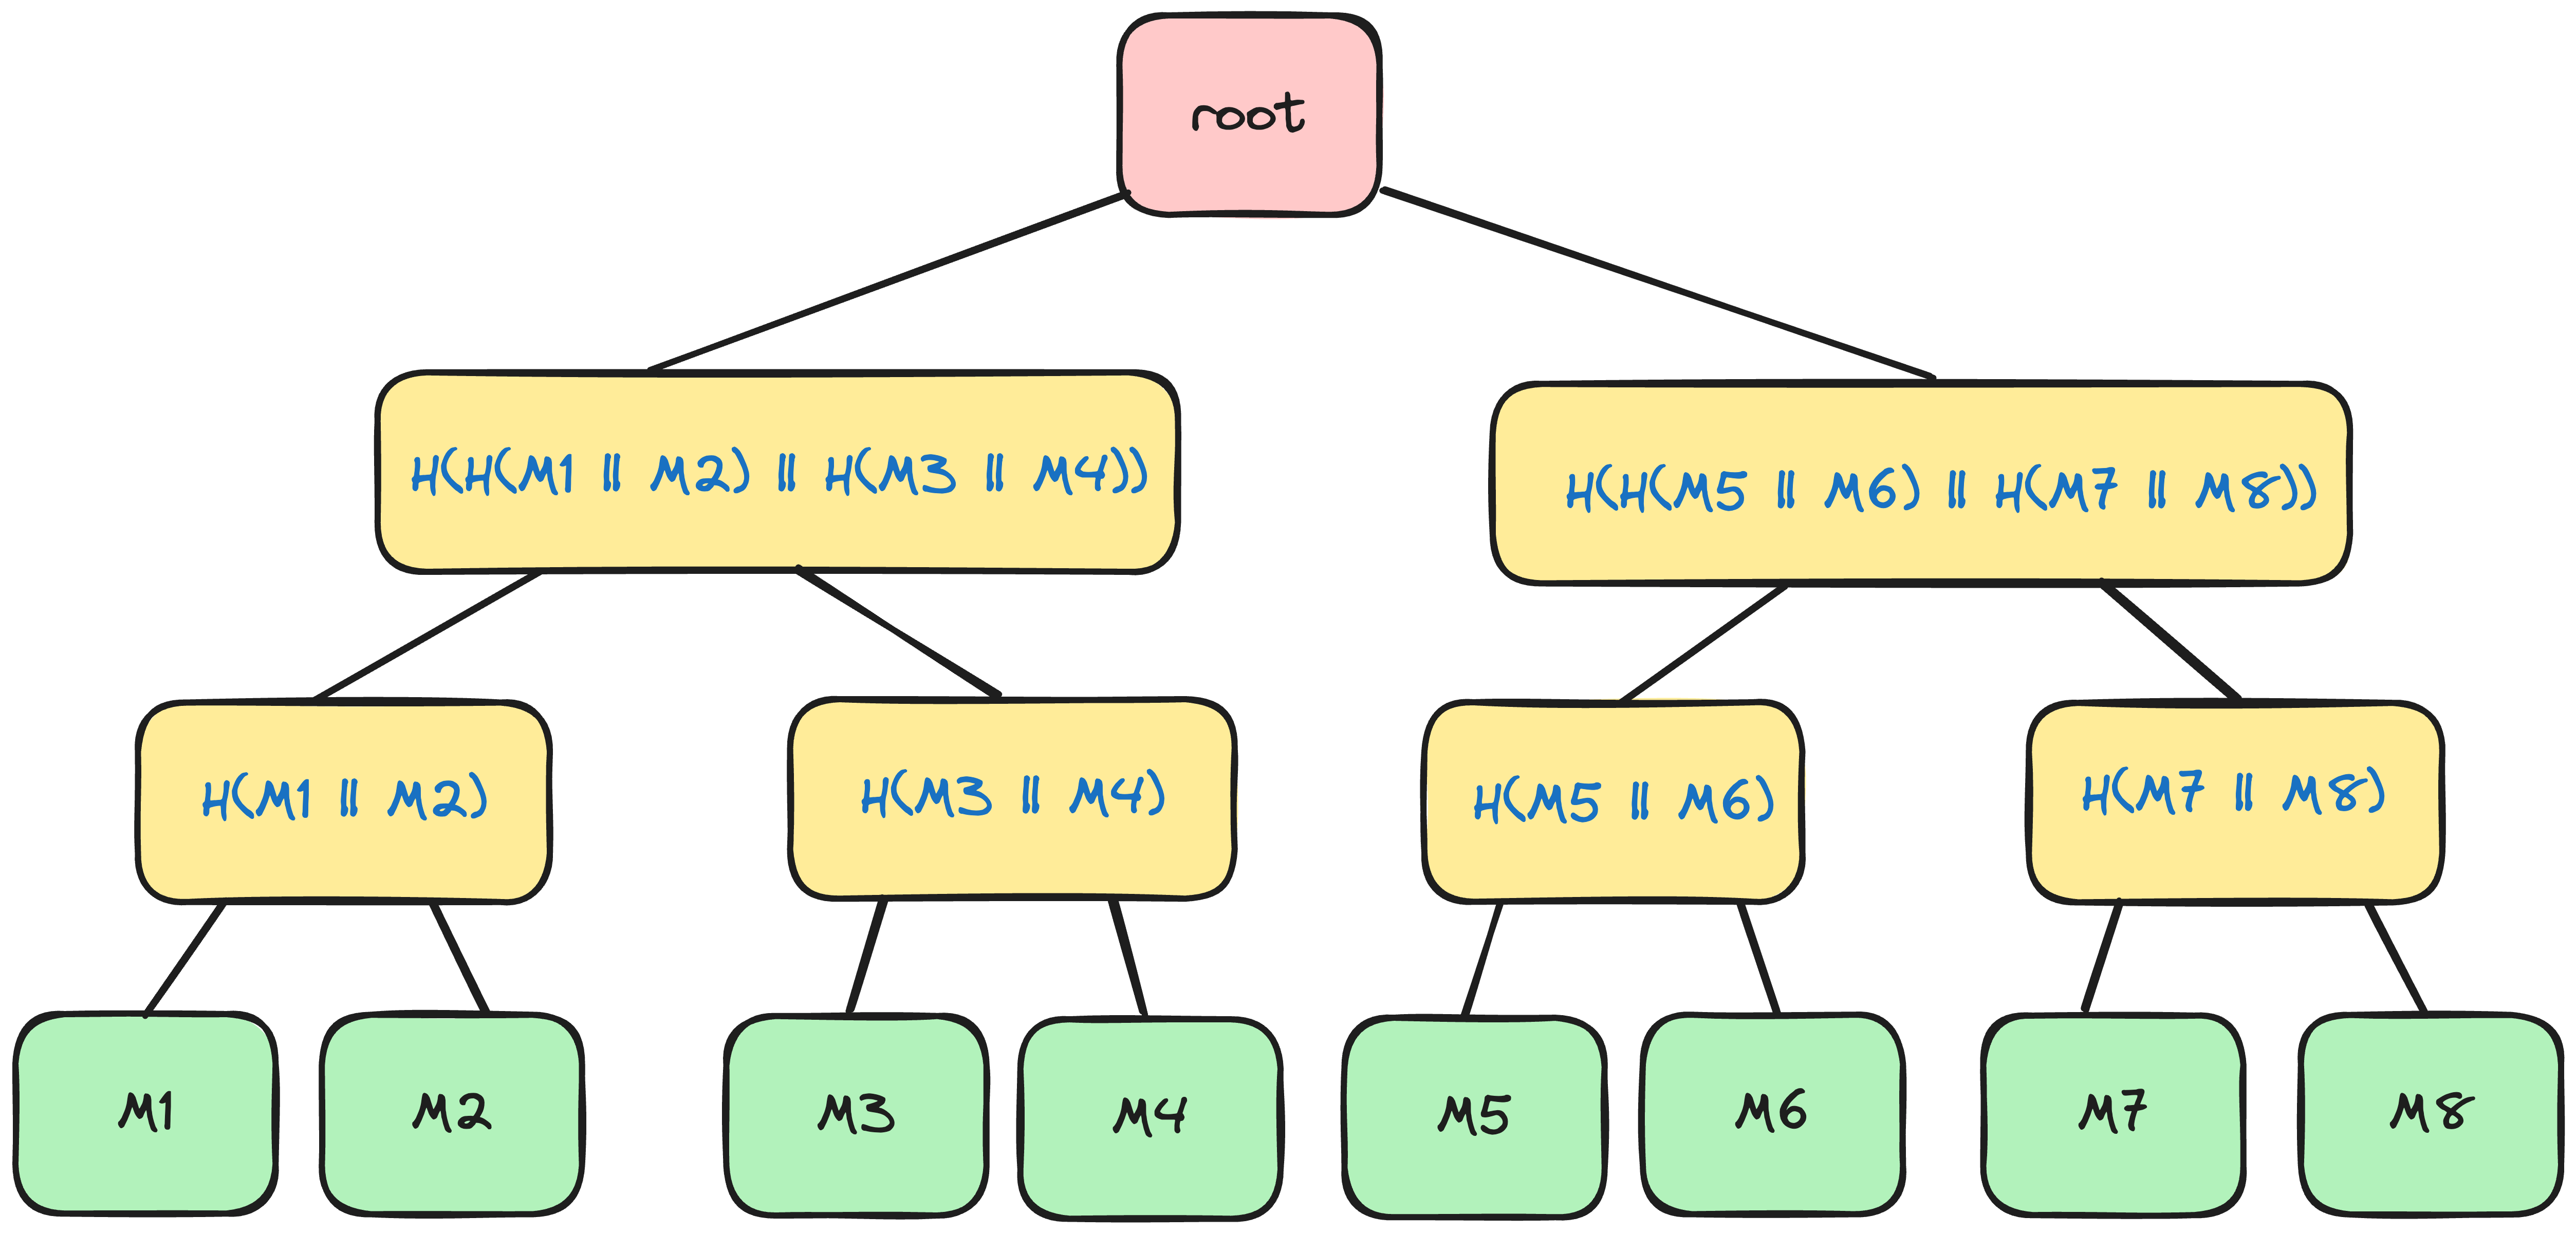
\includegraphics[width=0.9\linewidth, clip]{images/lecture_5/MerkleTree.png}

    \caption{Merkle Tree structure}
\end{figure}

A Merkle Tree is a data structure to efficiently and securely verify the commiments to a vector of data. It is a binary tree where each leaf node represents a hash of a data block, and each non-leaf node is a hash of its child nodes' concatenated hashes. The top node, called the root hash or Merkle root, uniquely represents the entire data set. By comparing this root with a known valid root, one can quickly verify the authenticity and integrity of the data without needing to examine the entire dataset. 

To prove the inclusion of element into the tree, a corresponding Merkle Branch is used. On the example below, $M_1$ inclusion is proved, and 
$(M_2, H(M_3 \parallel M_4), H(H(M_5 \parallel M_6) \parallel H(M_7 \parallel M_8)))$ is an inclusion branch vector.

\begin{figure}[H]
    \centering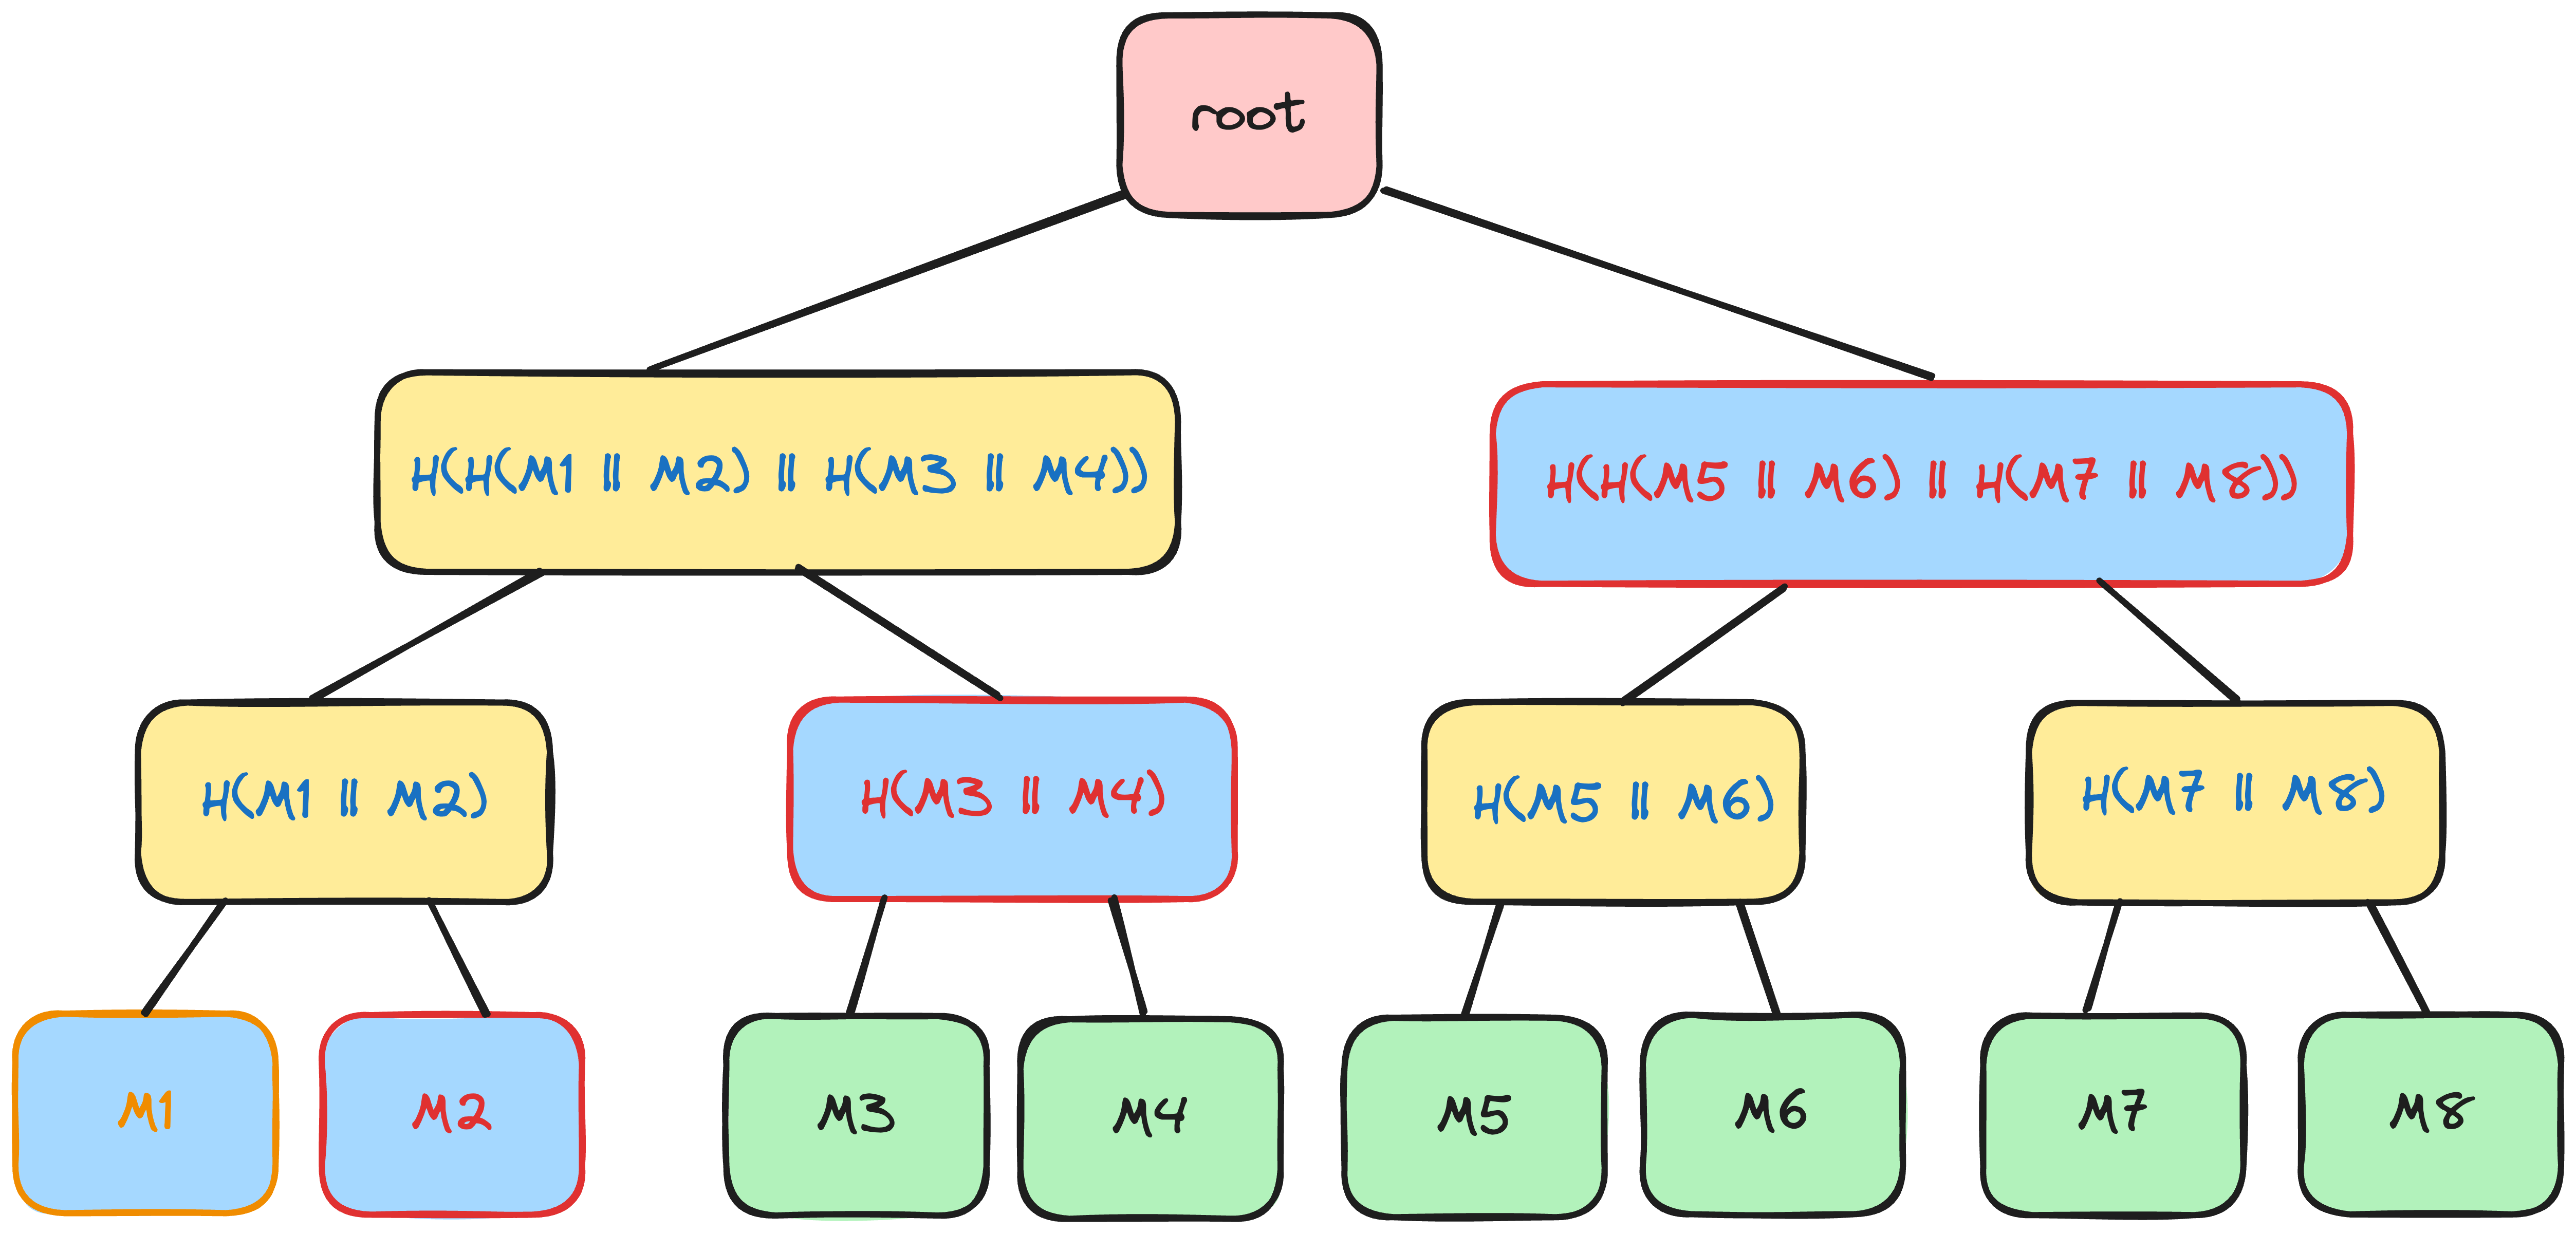
\includegraphics[width=0.9\linewidth, clip]{images/lecture_5/MerkleTreeProof.png}

    \caption{Merkle Tree inclusion proof branch}
\end{figure}

One of Merkle tree key advantages is that it allows for the selective disclosure of specific elements within the data set without revealing the rest. 

\subsection{Polynomial commitment}

Polynomial commitment can be used to prove that the commited polynomial satisfies certain properties $P(x_1, x_2, \ldots, x_n) = y$, without revealing what the polynomial is.
The commitment is generally succint, which means that it is much smaller than the polynomial it represents.

\textbf{The KZG polynomial commitment scheme}

The KZG (Kate-Zaverucha-Goldberg) is a polynomial commitment scheme:

\begin{enumerate}
    \item \textit{One-time ``Powers-of-tau`` trusted setup stage}. During trusted setup a set of elliptic curve points is generated. 
    Let $G$ be a generator point of some pairing-friendly
    elliptic curve group $\mathbb{G}$, $s$ some random value in the order of the $G$ point and $d$ be the maximum degree 
    of the polynomials we want to commit to.
    Public parameters of a trusted setup are calculated as:

    \vspace{-3mm}

    \begin{center}
        $[\tau^0]G, [\tau^1]G, \ldots, [\tau^d]G$
    \end{center}

    \vspace{-1mm}

    Parameter $\tau$ should be deleted after the ceremony. If it is revealed, the \textit{binding} property of the commitment scheme can be broken. 
    This parameter is usually called the \textit{toxic waste}.
    
    \item \textit{Commit to polynomial}. Given the polynomial $p(x) = \sum_{i = 0}^{d} p_i x^i$, compute the commitment $c = [p(\tau)]G $ 
    using the trusted setup. Although the committer cannot compute $p(\tau)$ directly since the value of $\tau$ is unknown, he can
    compute it using values $([\tau^0]G, [\tau^1]G, \ldots, [\tau^d]G)$:
    
    \vspace{-1mm}

    \begin{center}
       $ [p(\tau)]G = [\sum_{i=0}^{d} p_i \tau^i]G = \sum_{i=0}^{d}p_i[\tau^i]G$
    \end{center}
    
    \vspace{-1mm}

    \item \textit{Prove an evaluation}. To prove that at some point $x_0$ polynomial equals $y_0$ ($p(x_0) = y_0$), compute polynomial
    
    \vspace{-1mm}
    
    \begin{center}
        $q(x) = \frac{p(x) - y_0}{x - x_0}$.
    \end{center}

    \vspace{-1mm}

    Polynomial $q(x)$ is called ``quotient polynomial`` and only exists if and only if $p(x_0) = y_0$:
    \begin{enumerate}
        \item If $p(x_0) = y_0$, we define $r(x) := p(x) - y_0$;
        \item $r(x)$ has $x_0$ as a root, as $r(x_0) = 0$ by the definition. 
            That is why there exists $q(x)$, such that $r(x) = q(x)\cdot (x-x_0)$;
        \item Hence, the expression $q(x) = \frac{p(x) - y_0}{x-x_0}$ is a polynomial.
    \end{enumerate}
    
    The existance of this quotient polynomial serves
    as a proof of the evaluation. \textit{Prover} calculates proof $\pi = [q(\tau)]G$ and sends it to the \textit{Verifier}.

    \item \textit{Verify the proof}. Given a commitment $c = [p(\tau)]G$, an evaluation $p(x_0) = y_0$ and a proof $[q(\tau)]G$, we need to
    ensure that $q(\tau) \cdot (\tau - x_0) = p(\tau) - y_0$. This can be done using trusted setup without knowledge of $\tau$ using bilinear mapping:

    \vspace{-0.5mm}

    \begin{center}
        $e([q(\tau)]G_1, [\tau]G_2 - [x']G_2) = e([p(\tau)]G_1 - [y]G_1, G_2)$
    \end{center}
    
    \vspace{-1.5mm}

    Polynomial commiment schemes such as KZG are used in zero knowledge proof system to encode circuit constraints as a polynomial, 
    so that verifier could check random points to ensure that the constraints are met.

\end{enumerate}

\subsection{Exercises}

\vspace{-1mm}

\begin{xexercise}
    {Exercise 1.}
    {Dmytro and Denis were watching a horse race. Confident in
    his ability to predict the outcome, Dmytro decided to commit to his
    prediction. However, in his haste, he forgot to use a blinding factor. Now,
    Dmytro is concerned that Denis might discover his prediction before the race
    ends, which would defeat the purpose of his commitment.
    
    We define a dummy hash function $H: \mathbb{Z} \to \mathbb{F}_{41}$ as $H(x)
    = 13x+17$. Dmytro used a \textit{hash-based commitment} and $H$ as a hash
    function. The set of race horse numbers is $\{3, 5, 8, 15\}$. Help Denis to
    find out the horse number Dmytro have made a commitment to, if the
    commitment equals $C = 39$.}
    {4}
    {
        \item $3$.
        \item $5$.
        \item $8$.
        \item $15$.
    }
\end{xexercise}

\begin{xexercise}
    {Exercise 2.}
    {Denis made a setup (points $G$ and $U$) for a Pedersen
    commitment scheme and commited values $(m, r) = (3, 7)$ to Dmytro by sending him
    $C = [3]G + [7]U$. Dmytro did not verify the setup. Turns out that Denis knows
    that $U$ = $[6]G$. Denis is planning to send a different message from the one he
    originally committed to: $m_2 = 15$. Which values of $(m_2, r_2)$ should he send
    to Dmytro at the opening stage?}
    {4}
    {
        \item $(15, 5)$
        \item $(15, 7)$
        \item $(15, 4)$
        \item $(3, 5)$
    }
\end{xexercise}

\textbf{Exercise 3.} We define a dummy hash function $H: \mathbb{Z} \times
\mathbb{Z} \to \mathbb{F}_{41}$ as $H(x, y) = 3x+7y$. You have a Merkle tree
built with depth $4$ using the hash function $H$ with a root that equals $37$.
Which inclusion proof is valid for element $3$? Position defines how leaves
should be hashed:
\begin{itemize}
    \item if $\ell$, then $h_i \gets H(h_{i-1}, \mathsf{branch}[i])$,
    \item if $r$, then $h_i \gets H(\mathsf{branch}[i], h_{i-1})$.
\end{itemize}
\begin{enumerate}[(A)]
    \item Branch: $[4, 16, 13]$, Position: $[\ell,r,\ell]$
    \item Branch: $[1, 40, 3]$, Position: $[\ell, \ell, \ell]$
    \item Branch: $[5, 12, 13]$, Position: $[r, r, \ell]$
    \item Branch: $[4, 17, 13]$, Position: $[\ell, r, \ell]$
\end{enumerate}

\textbf{Exercise 4.} Given a polynomial $p(x) = x^3 - 10x^2 + 31x - 30$, Oleksandr wants to prove that $p(2)=0$. 
To do that, according to the KZG commitment scheme, he constructs the quotient polynomial $q(x)$ and wants 
to show that $q(\tau) \cdot (\tau - 2) = p(\tau)$. Assuming Oleksandr has conducted these steps correctly, 
what value of $q(x)$ has Oleksandr calculated?

\vspace{-3mm}

\begin{multicols}{2}
    \begin{enumerate}[(A)]
        \item $q(x) = 2x^2 + 4x - 6$
        \item $q(x) = x^3 - 10x^2 + 30x - 28$
        \item $q(x) = x^2 - 8x + 15$
        \item $q(x) = x^2 + 5x + 18$
    \end{enumerate}
\end{multicols}

\end{document}